\chapterimage{chapter_head_1.pdf} % Chapter heading image
\chapter{The way of the program}

The goal of this book is to teach you to think like a
computer scientist.  This way of thinking combines some of the best features
of mathematics, engineering, and natural science.  Like mathematicians,
computer scientists use formal languages to denote ideas (specifically
computations).  Like engineers, they design things, assembling components
into systems and evaluating tradeoffs among alternatives.  Like scientists,
they observe the behavior of complex systems, form hypotheses, and test
predictions.

\index{problem solving}

The single most important skill for a computer scientist is {\bf
	problem solving}.  Problem solving means the ability to formulate
problems, think creatively about solutions, and express a solution clearly
and accurately.  As it turns out, the process of learning to program is an
excellent opportunity to practice problem-solving skills.  That's why
this chapter is called, ``The way of the program.''

On one level, you will be learning to program, a useful
skill by itself.  On another level, you will use programming as a means to
an end.  As we go along, that end will become clearer.


\section{The Python programming language}
\index{programming language}
\index{language!programming}

The programming language you will learn is Python. Python is
an example of a {\bf high-level language}; other high-level languages
you might have heard of are C++, C\#, VB, JavaScript, and Java.

There are also {\bf low-level languages}, sometimes referred to as ``machine
languages'' or ``assembly languages.''  Loosely speaking, computers
can only execute programs written in low-level languages.  So
programs written in a high-level language have to be processed before
they can run.  This extra processing takes some time, which is a small
disadvantage of high-level languages.

\index{portability}
\index{high-level language}
\index{low-level language}
\index{language!high-level}
\index{language!low-level}

The advantages are enormous.  First, it is much easier for a human to program
in a high-level language.  Programs written in a high-level language
take less time to write, they are shorter and easier to read, and they
are more likely to be correct.  Second, high-level languages are {\bf
	portable}, meaning that they can run on different kinds of computers
with few or no modifications.  Low-level programs can run on only one
kind of computer and have to be rewritten to run on another.
Due to these advantages, almost all programs are written in high-level
languages.  Low-level languages are used only for a few specialized
applications.

\index{compile}
\index{interpret}

Two kinds of programs process high-level languages
into low-level languages: {\bf interpreters} and {\bf compilers}.
An interpreter reads a high-level program and executes it, meaning that it
does what the program says.  It processes the program a little at a time,
alternately reading lines and performing computations.


%MUST INCLUDE THE FIGURE HERE

\beforefig
\centerline{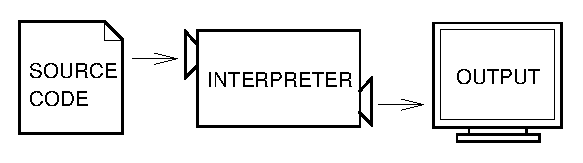
\includegraphics[height=0.77in]{figs/interpret.eps}}
\afterfig

\index{source code}
\index{object code}
\index{executable}

A compiler reads the program and translates it completely before the
program starts running.  In this context, the high-level program is
called the {\bf source code}, and the translated program is called the
{\bf object code} or the {\bf executable}.  Once a program is
compiled, you can execute it repeatedly without further translation.

\beforefig
\centerline{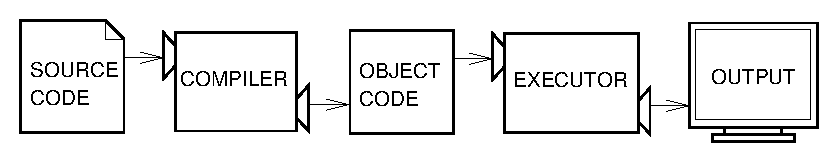
\includegraphics[height=0.77in]{figs/compile.eps}}
\afterfig

Python is considered an interpreted language because Python programs
are executed by an interpreter.  There are two ways to use the
interpreter: {\bf interactive mode} and {\bf script mode}. In
interactive mode, you type Python programs and the interpreter prints
the result:

\index{interactive mode}
\index{script mode}

\beforeverb
\begin{pyinterpreter}
>>> 1 + 1
2
\end{pyinterpreter}
\afterverb
%
The chevron, verb|>>>|, is the
{\bf prompt} the interpreter uses to indicate that it is ready.  If
you type {\tt 1 + 1}, the interpreter replies {\tt 2}.

\index{prompt}

Alternatively, you can store code in a file and use the interpreter to
execute the contents of the file, which is called a {\bf script}.  By
convention, Python scripts have names that end with {\tt .py}.
\index{script}
To execute the script, you have to tell the interpreter the name of
the file. In a Windows command shell, you would type {\tt python
	dinsdale.py}.  In other development environments, the details of
executing scripts are different.  You can find instructions for
your environment at the Python website \url{python.org}.

\index{testing!interactive mode}

Working in interactive mode is convenient for testing small pieces of
code because you can type and execute them immediately.  But for
anything more than a few lines, you should save your code
as a script so you can modify and execute it in the future.


\section{What is a program?}

A {\bf program} is a sequence of instructions that specifies how to
perform a computation.  The computation might be something
mathematical, such as solving a system of equations or finding the
roots of a polynomial, but it can also be a symbolic computation, such
as searching and replacing text in a document or (strangely enough)
compiling a program.

\index{program}

The details look different in different languages, but a few basic
instructions appear in just about every language:

\begin{description}
	
	\item[input:] Get data from the keyboard, a file, or some
	other device.
	
	\item[output:] Display data on the screen or send data to a
	file or other device.
	
	\item[math:] Perform basic mathematical operations like addition and
	multiplication.
	
	\item[conditional execution:] Check for certain conditions and
	execute the appropriate sequence of statements.
	
	\item[repetition:] Perform some action repeatedly, usually with
	some variation.
	
\end{description}

Believe it or not, that's pretty much all there is to it.  Every
program you've ever used, no matter how complicated, is made up of
instructions that look pretty much like these.  So you can think of
programming as the process of breaking a large, complex task
into smaller and smaller subtasks until the subtasks are
simple enough to be performed with one of these basic instructions.
\index{algorithm}
That may be a little vague, but we will come back to this topic
when we talk about {\bf algorithms}.

\section{What is debugging?}
\index{debugging}
\index{bug}

Programming is error-prone.  For whimsical reasons, programming errors
are called {\bf bugs} and the process of tracking them down is called
{\bf debugging}.
\index{debugging}
\index{bug}
Three kinds of errors can occur in a program: syntax errors, runtime 
errors, and semantic errors. It is useful
to distinguish between them in order to track them down more quickly.

\subsection{Syntax errors}
\index{syntax error}
\index{error!syntax}
\index{error message}

Python can only execute a program if the syntax is
correct; otherwise, the interpreter displays an error message.
{\bf Syntax} refers to the structure of a program and the rules about
that structure. \index{syntax} 
For example, parentheses have to come in matching pairs, so
{\tt (1 + 2)} is legal, but {\tt 1 + 2)} is a {\bf syntax error}.

\index{parentheses!matching}
\index{syntax}
\index{cummings, e. e.}

In English readers can tolerate most syntax errors, 
Python is not so forgiving.  If there is a single syntax error
anywhere in your program, Python will display an error message and quit,
and you will not be able to run your program. During the first few
weeks of your programming career, you will probably spend a lot of
time tracking down syntax errors.  As you gain experience, you will
make fewer errors and find them faster.

\subsection{Runtime errors}
\label{runtime}
\index{runtime error}
\index{error!runtime}
\index{exception}
\index{safe language}
\index{language!safe}

The second type of error is a runtime error, so called because the
error does not appear until after the program has started running.
These errors are also called {\bf exceptions} because they usually
indicate that something exceptional (and bad) has happened.
Runtime errors are rare in the simple programs you will see in the
first few chapters, so it might be a while before you encounter one.


\subsection{Semantic errors}
\index{semantics}
\index{semantic error}
\index{error!semantic}
\index{error message}

The third type of error is the {\bf semantic error}.  If there is a
semantic error in your program, it will run successfully in the sense
that the computer will not generate any error messages, but it will
not do the right thing.  It will do something else.  Specifically, it
will do what you told it to do.
The problem is that the program you wrote is not the program you
wanted to write.  The meaning of the program (its semantics) is wrong.
Identifying semantic errors can be tricky because it requires you to work
backward by looking at the output of the program and trying to figure
out what it is doing.

\subsection{Experimental debugging}

One of the most important skills you will acquire is debugging.
Although it can be frustrating, debugging is one of the most
intellectually rich, challenging, and interesting parts of
programming.

\index{experimental debugging}
\index{debugging!experimental}

In some ways, debugging is like detective work.  You are confronted
with clues, and you have to infer the processes and events that led
to the results you see.
Debugging is also like an experimental science.  Once you have an idea
about what is going wrong, you modify your program and try again.  If
your hypothesis was correct, then you can predict the result of the
modification, and you take a step closer to a working program.  If
your hypothesis was wrong, you have to come up with a new one.  As
Sherlock Holmes pointed out~\parencite{doyle2010sign}, ``When you have eliminated the
impossible, whatever remains, however improbable, must be the truth.''


For some people, programming and debugging are the same thing.  That
is, programming is the process of gradually debugging a program until
it does what you want.  The idea is that you should start with a
program that does {\em something} and make small modifications,
debugging them as you go, so that you always have a working program.

For example, Linux is an operating system that contains thousands of
lines of code, but it started out as a simple program Linus Torvalds
used to explore the Intel 80386 chip.  According to Larry Greenfield,
``One of Linus's earlier projects was a program that would switch
between printing AAAA and BBBB.  This later evolved to Linux.''
({\em The Linux Users' Guide} Beta Version 1).

\index{Linux}

Later chapters will make more suggestions about debugging and other
programming practices.

\section{Formal and natural languages}
\index{formal language}
\index{natural language}
\index{language!formal}
\index{language!natural}

\begin{definition}[Natural languages] are the languages people speak,
such as English, Spanish, and French.  They were not designed
by people (although people try to impose some order on them);
they evolved naturally.
\end{definition}

\begin{definition}[Formal languages] are languages that are designed by people for
specific applications.  For example, the notation that mathematicians
use is a formal language that is particularly good at denoting
relationships among numbers and symbols.  Chemists use a formal
language to represent the chemical structure of molecules.  And
most importantly:
\end{definition}

\begin{quote}
	{\bf Programming languages are formal languages that have been
		designed to express computations.}
\end{quote}

Formal languages tend to have strict rules about syntax.  For example,
$3 + 3 = 6$ is a syntactically correct mathematical statement, but 
$3 + = 6 \mbox{\pounds} 3$ is not. 
Syntax rules come in two flavors, pertaining to {\bf tokens} and
structure.  Tokens are the basic elements of the language, such as
words, numbers, operators.  One of the problems with $3 +
= 3 \mbox{\pounds} 6$ is that $\pounds$ is not a legal token in mathematics.

\index{token}
\index{structure}

The second type of syntax error pertains to the structure of a
statement; that is, the way the tokens are arranged.  The statement $3
+ = 6 - 3$ is illegal because even though $+$ and $=$ are
legal tokens, you can't have one right after the other.

When you read a sentence in English or a statement in a formal
language, you have to figure out what the structure of the sentence is
(although in a natural language you do this subconsciously).  This
process is called {\bf parsing}.

\index{parse}

For example, when you hear the sentence, ``The penny dropped,'' you
understand that ``the penny'' is the subject and ``dropped'' is the
predicate.  Once you have parsed a sentence, you can figure out what it
means, or the semantics of the sentence.  Assuming that you know
what a penny is and what it means to drop, you will understand the
general implication of this sentence.

Although formal and natural languages have many features in
common---tokens, structure, syntax, and semantics---there are some
important differences:

\index{ambiguity}
\index{redundancy}
\index{literalness}

\begin{description}
	
	\item[ambiguity:] Natural languages are full of ambiguity, which
	people deal with by using contextual clues and other information.
	Formal languages are designed to be nearly or completely unambiguous,
	which means that any statement has exactly one meaning,
	regardless of context.
	
	\item[redundancy:] In order to make up for ambiguity and reduce
	misunderstandings, natural languages employ lots of
	redundancy.  As a result, they are often verbose.  Formal languages
	are less redundant and more concise.
	
	\item[literalness:] Natural languages are full of idiom and metaphor.
	If I say, ``The penny dropped,'' there is probably no penny and
	nothing dropping\footnote{This idiom means that someone realized something
		after a period of confusion.}.  Formal languages
	mean exactly what they say.
	
\end{description}

Here are some suggestions for reading programs (and other formal
languages).  First, remember that formal languages are much more dense
than natural languages, so it takes longer to read them.  Also, the
structure is very important, so it is usually not a good idea to read
from top to bottom, left to right.  Instead, learn to parse the
program in your head, identifying the tokens and interpreting the
structure.  Finally, the details matter.  Small errors in
spelling and punctuation, which you can get away
with in natural languages, can make a big difference in a formal
language.

\section{The first program}
\label{hello}

\index{Hello, World}

Traditionally, the first program you write in a new language
is called ``Hello, World!'' because all it does is display the
words, ``Hello, World!''  In Python 3, it looks like this:

\beforeverb
\begin{pyinterpreter}
>>> print('Hello, World!')
Hello, World!
\end{pyinterpreter}
\afterverb
%

The quotation marks in the program mark the beginning and end
of the text to be displayed; they don't appear in the result.

\index{quotation mark}
\index{print statement}
\index{statement!print}

Some people judge the quality of a programming language by the
simplicity of the ``Hello, World!'' program.  By this standard, Python
does about as well as possible.


\section{Debugging}
\index{debugging}

It is a good idea to read this book in front of a computer so you can
try out the examples as you go.  You can run most of the examples in
interactive mode, but if you put the code into a script, it is easier
to try out variations.
Whenever you are experimenting with a new feature, you should try
to make mistakes.  For example, in the ``Hello, world!'' program,
what happens if you leave out one of the quotation marks?  What
if you leave out both?  What if you spell {\tt print} wrong?

\index{error message}

\begin{remark}
This kind of experiment helps you remember what you read; it also helps
with debugging, because you get to know what the error messages mean.
It is better to make mistakes now and on purpose than later
and accidentally.
\end{remark}

Programming, and especially debugging, sometimes brings out strong
emotions.  If you are struggling with a difficult bug, you might 
feel angry, despondent or embarrassed.
There is evidence that people naturally respond to computers as if
they were people\footnote{See Reeves and Nass, {\it The Media
		Equation: How People Treat Computers, Television, and New Media
		Like Real People and Places}.}.  
When they work well, we think
of them as teammates, and when they are obstinate or rude, we
respond to them the same way we respond to rude,
obstinate people.
Preparing for these reactions might help you deal with them.
One approach is to think of the computer as an employee with
certain strengths, like speed and precision, and
particular weaknesses, like lack of empathy and inability
to grasp the big picture.
Your job is to be a good manager: find ways to take advantage
of the strengths and mitigate the weaknesses.  And find ways
to use your emotions to engage with the problem,
without letting your reactions interfere with your ability
to work effectively.

Learning to debug can be frustrating, but it is a valuable skill
that is useful for many activities beyond programming.  At the
end of each chapter there is a debugging section, like this one,
with my thoughts about debugging.  I hope they help!


\section{Glossary}
	
\begin{vocabulary}[problem solving:]  
The process of formulating a problem, finding a solution, and expressing the solution.
	\index{problem solving}
\end{vocabulary}
	
\begin{vocabulary}[high-level language:]  A programming language like Python that
	is designed to be easy for humans to read and write.
	\index{high-level language}
\end{vocabulary}
	
\begin{vocabulary}[low-level language:]  A programming language that is designed
	to be easy for a computer to execute; also called ``machine language'' or
	``assembly language.''
	\index{low-level language}
\end{vocabulary}
	
\begin{vocabulary}[portability:]  A property of a program that can run on more
	than one kind of computer.
	\index{portability}
\end{vocabulary}
	
\begin{vocabulary}[interpret:]  To execute a program in a high-level language
	by translating it one line at a time.
	\index{interpret}
\end{vocabulary}
	
\begin{vocabulary}[compile:]  To translate a program written in a high-level language
	into a low-level language all at once, in preparation for later
	execution.
	\index{compile}
\end{vocabulary}
	
\begin{vocabulary}[source code:]  A program in a high-level language before
	being compiled.
	\index{source code}
\end{vocabulary}
	
\begin{vocabulary}[object code:]  The output of the compiler after it translates
	the program.
	\index{object code}
\end{vocabulary}
	
\begin{vocabulary}[executable:]  Another name for object code that is ready
	to be executed.
	\index{executable}
\end{vocabulary}
	
\begin{vocabulary}[prompt:] Characters displayed by the interpreter to indicate
	that it is ready to take input from the user.
	\index{prompt}
\end{vocabulary}
	
\begin{vocabulary}[script:] A program stored in a file (usually one that will be
	interpreted).
	\index{script}
\end{vocabulary}
	
\begin{vocabulary}[interactive mode:] A way of using the Python interpreter by
	typing commands and expressions at the prompt.
	\index{interactive mode}
\end{vocabulary}
	
\begin{vocabulary}[script mode:] A way of using the Python interpreter to read
	and execute statements in a script.
	\index{script mode}
\end{vocabulary}
	
\begin{vocabulary}[program:] A set of instructions that specifies a computation.
	\index{program}
\end{vocabulary}
	
\begin{vocabulary}[algorithm:]  A general process for solving a category of
	problems.
	\index{algorithm}
\end{vocabulary}
	
\begin{vocabulary}[bug:]  An error in a program.
	\index{bug}
\end{vocabulary}
	
\begin{vocabulary}[debugging:]  The process of finding and removing any of the
	three kinds of programming errors.
\end{vocabulary}
	
\begin{vocabulary}[syntax:]  The structure of a program.
	\index{syntax}
\end{vocabulary}
	
\begin{vocabulary}[syntax error:]  An error in a program that makes it impossible
	to parse (and therefore impossible to interpret).
	\index{syntax error}
\end{vocabulary}
	
\begin{vocabulary}[exception:]  An error that is detected while the program is running.
	\index{exception}
\end{vocabulary}
	
\begin{vocabulary}[semantics:]  The meaning of a program.
	\index{semantics}
\end{vocabulary}
	
\begin{vocabulary}[semantic error:]   An error in a program that makes it do something
	other than what the programmer intended.
	\index{semantic error}
\end{vocabulary}
	
\begin{vocabulary}[natural language:]  Any one of the languages that people speak that
	evolved naturally.
	\index{natural language}
\end{vocabulary}
	
\begin{vocabulary}[formal language:]  Any one of the languages that people have designed
	for specific purposes, such as representing mathematical ideas or
	computer programs; all programming languages are formal languages.
	\index{formal language}
\end{vocabulary}
	
\begin{vocabulary}[token:]  One of the basic elements of the syntactic structure of
	a program, analogous to a word in a natural language.
	\index{token}
\end{vocabulary}
	
\begin{vocabulary}[parse:]  To examine a program and analyze the syntactic structure.
	\index{parse}
\end{vocabulary}
	
\begin{vocabulary}[print statement:]  An instruction that causes the Python
	interpreter to display a value on the screen.
	\index{print statement}
	\index{statement!print}
\end{vocabulary}


\section{Exercises}

\begin{exercise}
	Use a web browser to go to the Python website \url{python.org}.
	This page contains information about Python and links
	to Python-related pages, and it gives you the ability to search
	the Python documentation.
	
	For example, if you enter {\tt print} in the search window, the
	first link that appears is the documentation of the {\tt print}
	statement.  At this point, not all of it will make sense to you,
	but it is good to know where it is.
	
	\index{documentation}
	\index{python.org}
\end{exercise}

\begin{exercise}
	Start the Python interpreter and type {\tt help()} to start the online
	help utility.  Or you can type \verb"help('print')" to get information
	about the {\tt print} statement.
	
	If this example doesn't work, you
	may need to install additional Python documentation or set an
	environment variable; the details depend on your operating system and
	version of Python.
	%
	\index{help utility}
\end{exercise}

\begin{exercise}
	Start the Python interpreter and use it as a calculator.
	Python's syntax for math operations is almost the same as
	standard mathematical notation.  For example, the symbols
	{\tt +}, {\tt -} and {\tt /} denote addition, subtraction
	and division, as you would expect.  The symbol for
	multiplication is {\tt *}.
	
	If you run a 10 kilometer race in 43 minutes 30 seconds, what is your
	average time per mile?  What is your average speed in miles per hour?
	(Hint: there are 1.61 kilometers in a mile).
	%
	\index{calculator}
	\index{running pace}
	
\end{exercise}
